\normaltrue
\correctionfalse

%\UPSTIidClasse{12} % 11 sup, 12 spé
%\newcommand{\UPSTIidClasse}{12}

%\exer{Passerelle$\star$ \label{C2:10:Coh:529}}
\subsection*{Passerelle$\star$ \label{C2:10:Coh:529}}
\setcounter{question}{0}
\marginnote{\xpComp{RDM}{01}}%\UPSTIcompetence[2]{C2-10}
\index{Compétence C2-10}\index{Compétence RDM-01}
\index{Torseur de cohésion}
\index{Diagramme des efforts intérieurs}

\ifcorrection
\else
\marginnote{\textbf{Pas de corrigé pour cet exercice.}}
\fi



\begin{marginfigure}
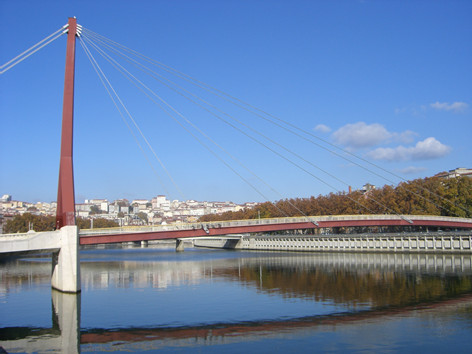
\includegraphics[width=\linewidth]{529_01}

\caption{Passerelle réelle}
\end{marginfigure}

\begin{marginfigure}
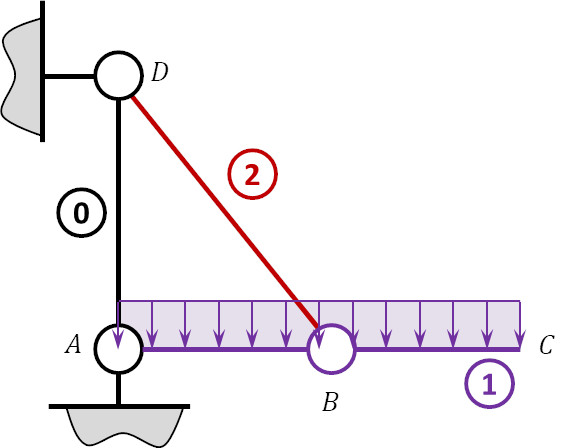
\includegraphics[width=\linewidth]{529_02}

\caption{Modèle choisi}
\end{marginfigure}

On s'intéresse au dimensionnement des haubans \textbf{(2)} permettant de maintenir en équilibre une passerelle.
On modélise la charge sur le pont comme une charge linéique~$c$. On note $L = AB = BC$. On note $\ell = BD$.

\subsection*{Détermination du torseur de cohésion}
\question{Réaliser le paramétrage du problème.}
\ifprof
\begin{corrige}~\\
\end{corrige}
\else
\fi

\question{Déterminer les actions mécaniques dans les liaisons.}
\ifprof
\begin{corrige}~\\
\end{corrige}
\else
\fi

\question{Déterminer le torseur de cohésion dans les poutres \textbf{(1)} et \textbf{(2)}.}
\ifprof
\begin{corrige}~\\
\end{corrige}
\else
\fi

\question{Tracer les diagrammes des sollicitations.}
\ifprof
\begin{corrige}~\\
\end{corrige}
\else
\fi


\subsection*{Déformation du hauban et déplacement de la structure}
On considère ici que le pont (1) est indéformable, mais que le hauban (2) est déformable. 

\question{Déterminer l'allongement du câble.}
\ifprof
\begin{corrige}~\\
\end{corrige}
\else
\fi

\question{En faisant l'hypothèse que la rotation de la passerelle en $A$ est << petite >>, déterminer le déplacement du point $B$ puis du point $C$. }
\ifprof
\begin{corrige}~\\
\end{corrige}
\else
\fi

\subsection*{Moment quadratique}
\begin{marginfigure}
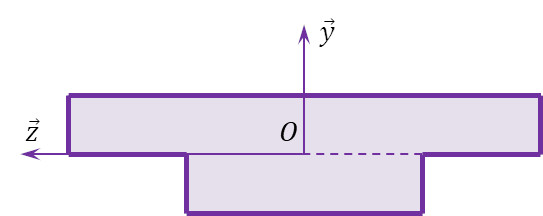
\includegraphics[width=\linewidth]{529_03}

\caption{Section de la passerelle}
\end{marginfigure}
La section de la passerelle est donnée figure suivante. 

\question{Déterminer le moment quadratique en $O$ par rapport à $\vect{y}$ puis par rapport à $\vect{z}$. }




\ifprof
\else

\marginnote{Corrigé voir \ref{C2:10:Coh:529}.}

\fi

